% This is samplepaper.tex, a sample chapter demonstrating the
% LLNCS macro package for Springer Computer Science proceedings;
% Version 2.20 of 2017/10/04
%
\documentclass[runningheads]{llncs}
%
\usepackage{graphicx}
\usepackage{url}
\usepackage[scale=0.67]{geometry}
% Used for displaying a sample figure. If possible, figure files should
% be included in EPS format.
%
% If you use the hyperref package, please uncomment the following line
% to display URLs in blue roman font according to Springer's eBook style:
% \renewcommand\UrlFont{\color{blue}\rmfamily}

\begin{document}
%
\title{Proposition de poster : un simulateur de Machines de Turing en ligne, utilisé pour des cours d'informatique sur la calculabilité et la complexité}%\thanks{Supported by ENS Rennes and CentraleSup{\'e}lec.}}
%
\titlerunning{Proposition de poster : utilisation d'un simulateur de Machines de Turing}
% % If the paper title is too long for the running head, you can set
% % an abbreviated paper title here
% %
% \author{Lilian Besson\inst{1}\orcidID{0000-0003-2767-2563}}
% %
% \authorrunning{Lilian Besson}
% % First names are abbreviated in the running head.
% % If there are more than two authors, 'et al.' is used.
% %
% \institute{{\'E}cole Normale Sup{\'e}rieure de Rennes, Bruz, France\\
% \email{lilian.besson{@}ens-rennes.fr}\\
% \url{www.ens-rennes.fr/}}
%
\maketitle              % typeset the header of the contribution
%
\begin{abstract}
    % The abstract should briefly summarize the contents of the paper in 150--250 words.
    % https://www.didapro.org/8/contributions-dates/
    Je propose un poster, qui présentera un simulateur de Machines de Turing, disponible en ligne (sur la page \url{naereen.github.io/jsTuring_fr/turing.html}),
    qui a été utilisé avec succès pour un cours introduisant la calculabilité et la complexité dans une école d'ingénieurs en France,
    ainsi qu'un cours de Master pour des étudiants préparant l'option majeure en informatique à l'examen national de mathématiques de l'agr{\'e}gation.
    L'affiche détaillera l'interface utilisateur du simulateur de la machine de Turing et explique ces deux utilisations réussies.

    \keywords{Machines de Turing \and Outil en ligne pour enseigner l'informatique théorique \and Javascript \and Outil open-source.}
\end{abstract}
%
%
%

% -------------------------
\section*{Aperçu du contenu de l'affiche}

L'affiche présentera les points suivants.

\subsection*{Présentation de la machine de Turing}

J'introduis rapidement les notations du modèle de machines de Turing, en utilisant les notations modernes \cite{turingmachine}, et non les notations historiques de Turing (1936).
%
Une machine de Turing (à bande unique) peut être formellement définie comme un 7-uplet $M=\langle Q,\Gamma \, b,\Sigma \,, \delta , q_{0},F\rangle$, où

\begin{small}
\begin{itemize}
    \item
    $Q$ est un ensemble fini et non vide d'états ;
    \item
    $\Gamma$ est un ensemble fini et non vide de symboles alphabétiques ;
    \item
    $b\in \in \Gamma$ est le symbole vide (le seul symbole autorisé à apparaître sur la bande infiniment souvent à n'importe quelle étape du calcul) ;
    \item
    $\Sigma \subseteq \Gamma \Gamma \setminus \{b\}$ est l'ensemble des symboles d'entrée, c'est-à-dire l'ensemble des symboles autorisés à apparaître dans le contenu initial de la bande ;
    \item
    $q_{0}\in Q$ est l'état initial ;
    \item
    $F\subseteq Q$ est l'ensemble des états finaux ou des états acceptants. Le contenu initial de la bande est dit accepté par $M$ s'il s'arrête finalement dans un état à partir de $F$.
    \item
    $\delta :(Q\setminus F)\times \Gamma \not \not \time \to Q\times \Gamma \times \L,R\}$ est une fonction partielle appelée fonction de transition, où L est décalage gauche, R est décalage droit. Si $\delta$ n'est pas défini sur l'état courant et le symbole de bande courant, alors la machine s'arrête.
\end{itemize}
\end{small}


\subsection*{Présentation du simulateur de machines de Turing en ligne}

Le simulateur de la machine de Turing présenté \cite{morphett_simulators,naereen_simulators},
peut être consulté en ligne à l'adresse suivante
\url{morphett.info/turing/} en anglais,
et \url{naereen.github.io/jsTuring_fr/} en français.
%
En incluant deux captures d'écran du simulateur, nous présentons les différents composants d'une machine de Turing (bande, état, mot d'entrée, table de transition, etc), voir Figure~\ref{fig:screenshots}.
Nous présentons également l'interface utilisateur, qui permet d'enregistrer une machine décrite par sa table de transition $\delta$ dans un fichier en ligne (en utilisant les gists anonymes de GitHub, \url{gist.github.com/}), et de charger des machines déjà écrites.

\begin{figure}[!h]
    \centering
    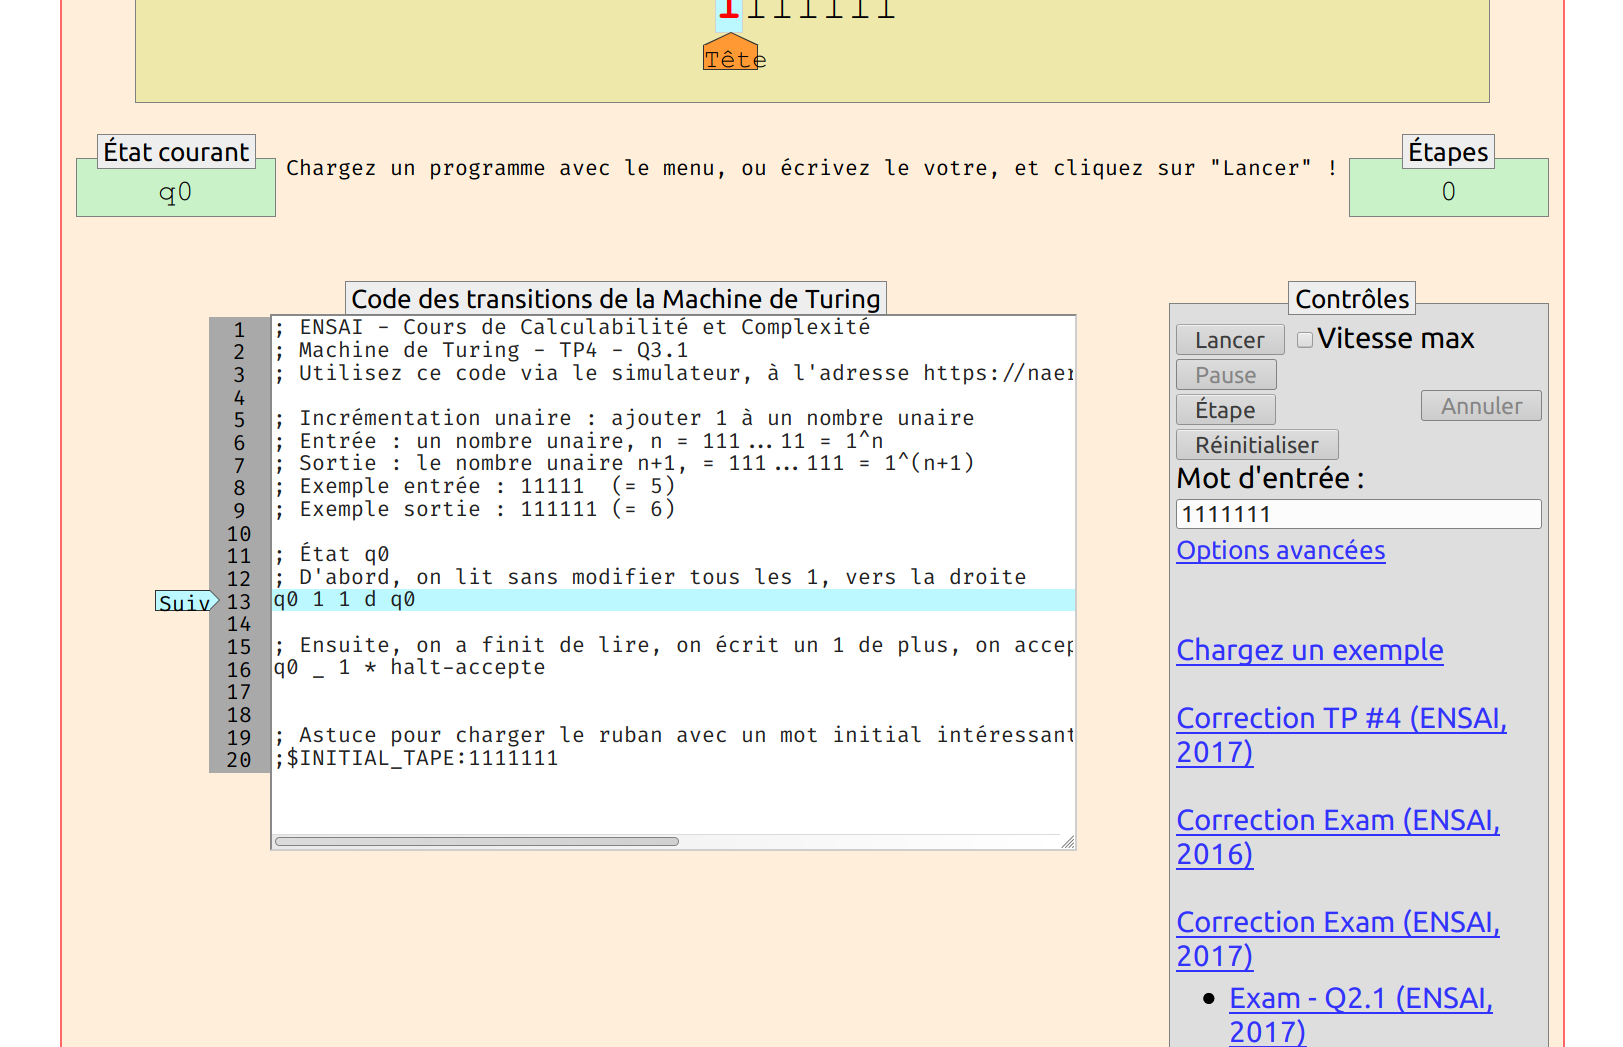
\includegraphics[width=0.49\textwidth]{interactive_Turing_Machine_simulator_1.png}
    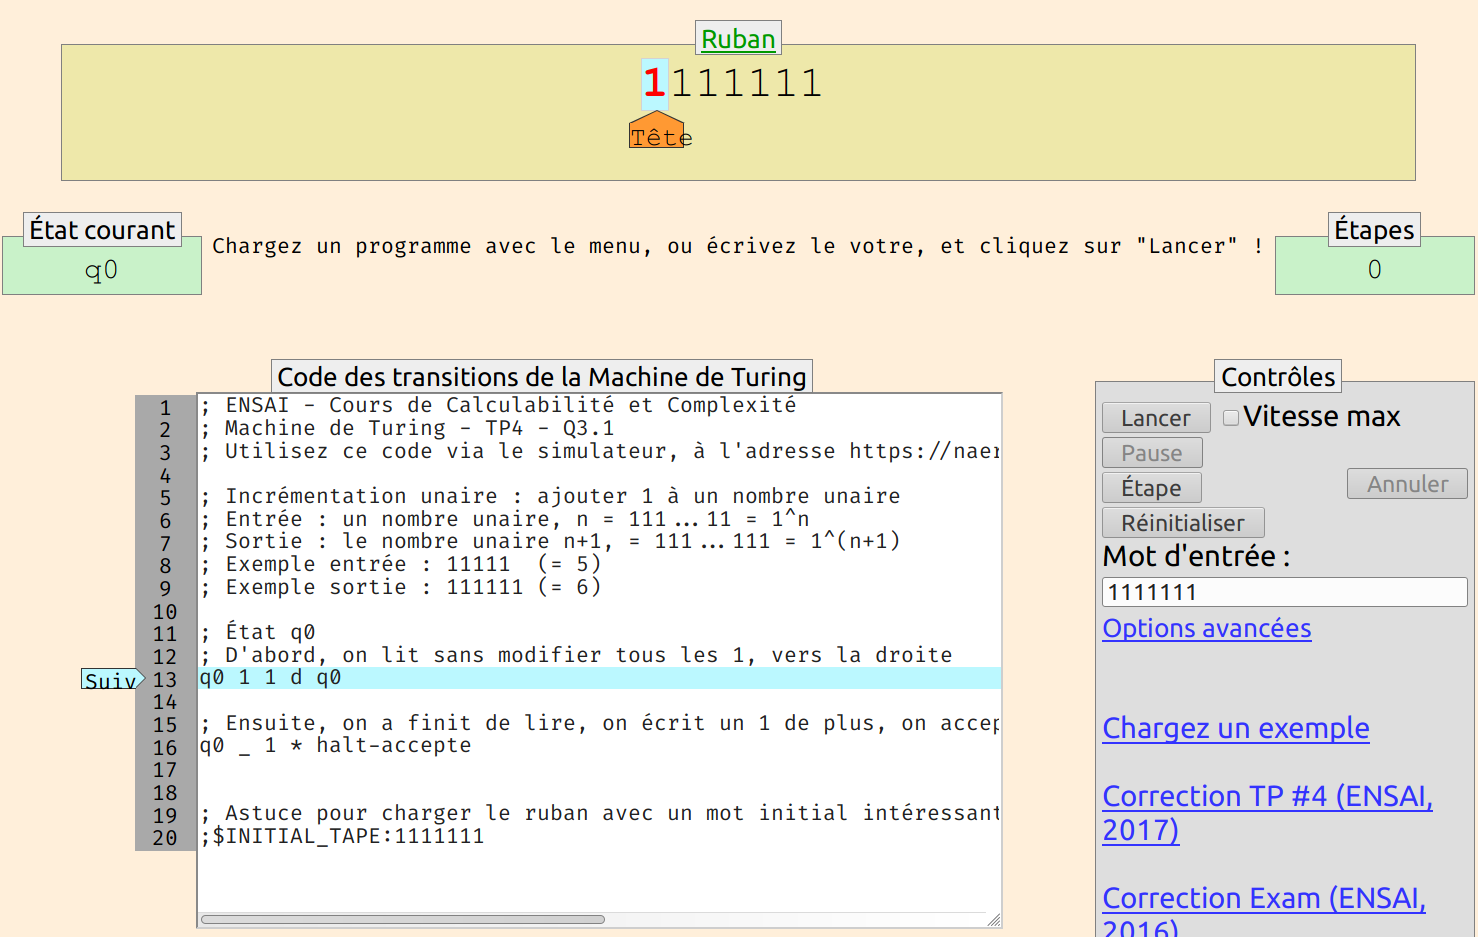
\includegraphics[width=0.49\textwidth]{interactive_Turing_Machine_simulator_2.png}
    \caption{Captures d'écran de l'interface utilisateur du simulateur en ligne de la machine de Turing \url{naereen.github.io/jsTuring_fr/turing.html}.}
    \label{fig:screenshots}
\end{figure}


\subsection*{Cas d'utilisation pour l'enseignement}

En permettant de charger des exemples de machines de Turing  pré-écrits, le simulateur a été utilisé avec succès dans des travaux pratiques pour deux classes différentes depuis 2017.


\paragraph{Une curiosité}

La dernière partie du poster détaillera le cas intéressant de la \emph{machine de Turing universelle}, pour attiser la curiosité des participants à la conférence.


% ---- Bibliography ----
%
% BibTeX users should specify bibliography style 'splncs04'.
% References will then be sorted and formatted in the correct style.
%
% \bibliographystyle{splncs04}
% \bibliography{mybibliography}
%
\begin{thebibliography}{8}
    \bibitem{turingmachine}
    Wikipedia contributors.
    \textbf{Turing Machine}, consulté en octobre 2019.
    \url{en.wikipedia.org/wiki/Turing_machine}.

    \bibitem{morphett_simulators}
    \textbf{Turing machine simulator},
    écrit par Anthony Morphett.
    Code source sur \url{github.com/awmorp/jsturing},
    interface web à \url{morphett.info/turing/}.

    \bibitem{naereen_simulators}
    \textbf{Simulateur de Machines de Turing},
    traduit par Lilian Besson.
    Code source sur \url{github.com/Naereen/jsTuring_fr},
    interface web à \url{naereen.github.io/jsTuring_fr/turing.html}.
\end{thebibliography}
\end{document}
